\begin{activity}{Structures and Steady-State Fields}

\section*{Purpose}
Gravity and magnetics activities in this course have had you sketch fields around simple structures -- a sphere, a dike, a fault -- and reason about the pattern from first principles before any computation. This activity does the same for heat conduction: given a structure of different conductivity than its surroundings, sketch the isotherms (temperature field) and heat flux lines (analogous to field lines) around it, in steady state, with no internal heat production anywhere.

\section*{Learning Outcomes}
By the end of this activity, you should be able to:
\begin{itemize}
  \item Sketch how isotherms and flux lines distort around a body of different thermal conductivity than its host.
  \item Explain why flux lines bend toward the higher-conductivity path, and connect this to the same refraction principle already used for electrical current and (in Week 6) magnetic field lines.
  \item Distinguish a field distorted by a \emph{material property} contrast (conductivity) from one distorted by a \emph{boundary geometry} effect (topography), using the same steady-state machinery for both.
\end{itemize}

\section*{Background}
In steady state with no internal heat production, two conditions hold at any interface between different conductivities:
\begin{itemize}
  \item Temperature is continuous across the boundary (no physical jump).
  \item The heat flux \emph{normal} to the boundary is continuous (nothing is accumulating there).
\end{itemize}
Just as electrical current refracts at a resistivity contrast, and magnetic field lines refract at a susceptibility contrast, heat flux lines refract at a conductivity contrast -- bending toward whichever side lets more flux pass for the same driving gradient. None of the three structures below has any internal heat production; the only thing distorting each field is either a conductivity contrast or, in the third case, the shape of the surface itself.

\section*{Tasks}
\begin{questions}

\question{A Pluton}

A circular pluton of lower conductivity than its host sits in otherwise uniform crust, far from any other structure. Regional heat flow $q$ points toward the surface, undisturbed far from the pluton (dashed lines).

\begin{center}
\begin{tikzpicture}[x=1cm,y=1cm]
  \draw[thick] (0,0) rectangle (10,8);
  \foreach \y in {0.7,1.4,2.1} \draw[dashed,gray] (0,\y) -- (10,\y);
  \foreach \y in {5.9,6.6,7.3} \draw[dashed,gray] (0,\y) -- (10,\y);
  \draw[thick] (5,4) circle (1.3);
  \node at (5,4) {$k_p < k_h$};
  \draw[->, thick] (-0.8,3.5) -- (-0.8,4.5);
  \node[left, font=\scriptsize] at (-0.9,4) {$q$};
  \node[above] at (5,8) {surface};
\end{tikzpicture}
\end{center}

\begin{enumerate}[label=(\alph*)]
  \item Sketch flux lines through the whole panel, including through and around the pluton. Do they concentrate into the pluton, or avoid it?
  \answerbox[2cm]

  \item Sketch isotherms consistent with your flux lines. Where are they compressed (steep gradient), and where are they spread out (gentle gradient)?
  \answerbox[2cm]

  \item If $k_p$ were \emph{greater} than $k_h$ instead, without redrawing, describe how your answer to (a) would change.
  \answerbox[2cm]
\end{enumerate}

\question{A Dike}

A near-vertical dike of higher conductivity than its host cuts across the same regional field.

\begin{center}
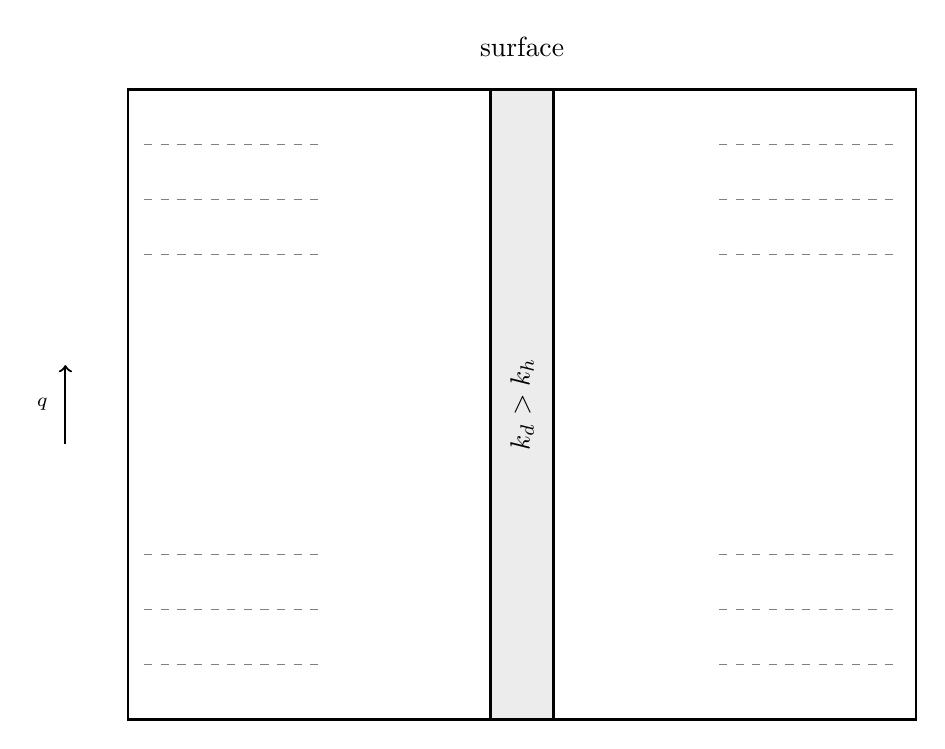
\begin{tikzpicture}[x=1cm,y=1cm]
  \draw[thick] (0,0) rectangle (10,8);
  \foreach \y in {0.7,1.4,2.1} \draw[dashed,gray] (0.2,\y) -- (2.5,\y);
  \foreach \y in {0.7,1.4,2.1} \draw[dashed,gray] (7.5,\y) -- (9.8,\y);
  \foreach \y in {5.9,6.6,7.3} \draw[dashed,gray] (0.2,\y) -- (2.5,\y);
  \foreach \y in {5.9,6.6,7.3} \draw[dashed,gray] (7.5,\y) -- (9.8,\y);
  \draw[thick, fill=gray!15] (4.6,0) -- (5.4,0) -- (5.4,8) -- (4.6,8) -- cycle;
  \node[rotate=90] at (5,4) {$k_d > k_h$};
  \draw[->, thick] (-0.8,3.5) -- (-0.8,4.5);
  \node[left, font=\scriptsize] at (-0.9,4) {$q$};
  \node[above] at (5,8.3) {surface};
\end{tikzpicture}
\end{center}

\begin{enumerate}[label=(\alph*)]
  \item Sketch flux lines through the panel. Does flux concentrate into the dike or avoid it -- and is that the same answer as Question 1, or the opposite?
  \answerbox[2cm]

  \item Sketch isotherms consistent with your flux lines. Would a borehole drilled straight down just outside the dike measure a different near-surface gradient than one drilled far away?
  \answerbox[2.5cm]
\end{enumerate}

\question{A Triangular Mountain}

Uniform crust, uniform conductivity throughout -- but the surface itself is not flat. Deep, undisturbed isotherms are shown; the surface follows the topographic profile.

\begin{center}
\begin{tikzpicture}[x=1cm,y=1cm]
  \draw[thick] (0,3) -- (0,0) -- (10,0) -- (10,3) -- (7,3) -- (5,7) -- (3,3) -- cycle;
  \foreach \y in {0.5,1.1,1.7} \draw[dashed,gray] (0,\y) -- (10,\y);
  \node[above] at (5,7) {peak};
\end{tikzpicture}
\end{center}

\begin{enumerate}[label=(\alph*)]
  \item Sketch isotherms from the deep, undisturbed region up through the topography, including beneath the peak itself. Do they stay flat all the way to the surface, or bend to follow the topographic profile?
  \answerbox[2.5cm]

  \item This distortion has nothing to do with a conductivity contrast -- conductivity is uniform everywhere in this panel. What, physically, is causing the isotherms to bend?
  \answerbox[2cm]

  \item At what distance from the peak (roughly, in mountain-heights) would you expect this distortion to have mostly died away? Compare your reasoning to how gravity and magnetic anomalies decay with distance from a source.
  \answerbox[2cm]
\end{enumerate}

\end{questions}

\section*{Key Ideas}

\textbf{Flux lines refract at a conductivity contrast, always bending toward the path that carries more flux for less resistance.} This is the same principle as electrical current refraction and magnetic field refraction -- a conductivity contrast, a resistivity contrast, and a susceptibility contrast all distort their respective fields the same way, for the same underlying reason.

\textbf{Whether flux concentrates into or avoids a structure depends on whether that structure is higher or lower conductivity than its host} -- a dike (high $k$) draws flux in; a pluton (low $k$, as drawn here) pushes flux around it. Reversing the contrast reverses the pattern.

\textbf{Not every field distortion comes from a material contrast.} The mountain's isotherms bend because the boundary condition itself (the surface, where $T=T_0$) is not flat -- the same kind of geometric effect that produces terrain corrections in gravity and magnetics, distinct from (and addable to) any density, susceptibility, or conductivity contrast in the subsurface.

\end{activity}
